% !TEX root = ../main.tex
% Einleitung

Das Bedürfnis, Informationen anschaulich darzustellen, ist ein Phänomen, das die Kulturgeschichte des Menschen seit der Frühzeit begleitet.
Eine der ältesten visuellen Metaphern ist der Baum.
So beschreibt Lima im Vorwort seines Buches \emph{The book of trees: Visualizing branches of knowledge} den Baum als einen "`visuellen Archetypen"' \footnote{ "`(...)the tree as one of the most popular, captivating, and widespread visual archetypes."' \cite[S. 9]{lima2014book}}. \\
Der Baum dient als Vorlage, um unterschiedlichste Zusammenhänge grafisch darzustellen.
Das Spektrum reicht von nahezu realistischen Darstellungen bis hin zu abstrakten Formen, reduziert auf Knoten und Kanten.
Als visuelle Metapher zur Darstellung von Informationen kommen Baumdiagramme in vielen Bereichen zum Einsatz; z.\,B. zur Darstellung von Erbfolgen, beim sogenannten Stammbaum, oder um Rangordnungen im Tierreich abzubilden. \cite{lima2014book}

Im Besonderen macht sich diese Darstellungsform die Hierarchie und geordnete Struktur eines Baumes zu Nutzen.
So lässt sich der Baum als eine visuelle Repräsentation verstehen, mit deren Hilfe sich komplexe Beziehungen zwischen einzelnen Entitäten übersichtlich darstellen lassen \cite[S. 43]{lima2014book}.

Die vorliegende Arbeit beschäftigt sich mit der visuellen Metapher des Baumes als eine Möglichkeit zur Darstellung der Kategorienstruktur der Wikipedia und versucht die Ähnlichkeiten zwischen Artikeln auf Paragrafenebene innerhalb eines Themenbereichs visuell kenntlich zu machen.
So zielt diese Arbeit darauf ab, die inhaltlichen Zusammenhänge der Themengebiete der Enzyklopädie Wikipedia grafisch darzustellen.
Dem Nutzer wird damit die Möglichkeit gegeben, die Darstellung flexibel, interaktiv und in Echtzeit nach seinen Intentionen bzw. Parametern zu verändern.

\section{Motivation}\label{subchap:motivation}
Als weiterführende Forschung beruht diese Arbeit auf den gewonnenen Erkenntnissen aus dem Projekt \emph{Visual Text Analytics}, entstanden an der Fakultät Medien der Bauhaus-Universität Weimar am Lehrstuhl Virtuelle Realität.
Dieses Projekt setzte sich bereits zum Ziel, die Ähnlichkeiten zwischen den Artikeln der Wikipedia zu visualisieren.
In der Darstellung werden die Artikel als Knoten umgesetzt, wohingegen die Kanten eine vorhandene Ähnlichkeit zwischen zwei Artikeln abbilden \cite{riehmann2016visualizing}.

Die Intention des Projekts bestand darin, die inhaltlichen Überschneidungen einer möglichst großen Anzahl von Wikipedia-Artikeln auf Grundlage ihrer Ähnlichkeitswerte, wie in der Abbildung \ref{fig:vta-cover} zu sehen, darzustellen.
Im Voraus wird ein Schwellwert für die Ähnlichkeitswerte zwischen den Artikeln festgelegt, welcher maßgeblich die Anordnung der Artikel in der Visualisierung bestimmt.
Ähnlichkeitswerte unter dem Schwellwert werden nicht mit einbezogen und folglich nicht dargestellt. 
Die auf diese Weise gefilterten, oberhalb des Schwellwerts liegenden Artikel werden dabei in Gruppen von ähnlichen Artikeln, sogenannten Clustern, zusammengefasst.
\footnote{Im Kapitel \ref{subchap:simmatrix} wird im Detail auf die Berechnung der Ähnlichkeiten eingegangen.}

\begin{figure}[ht]
\centering
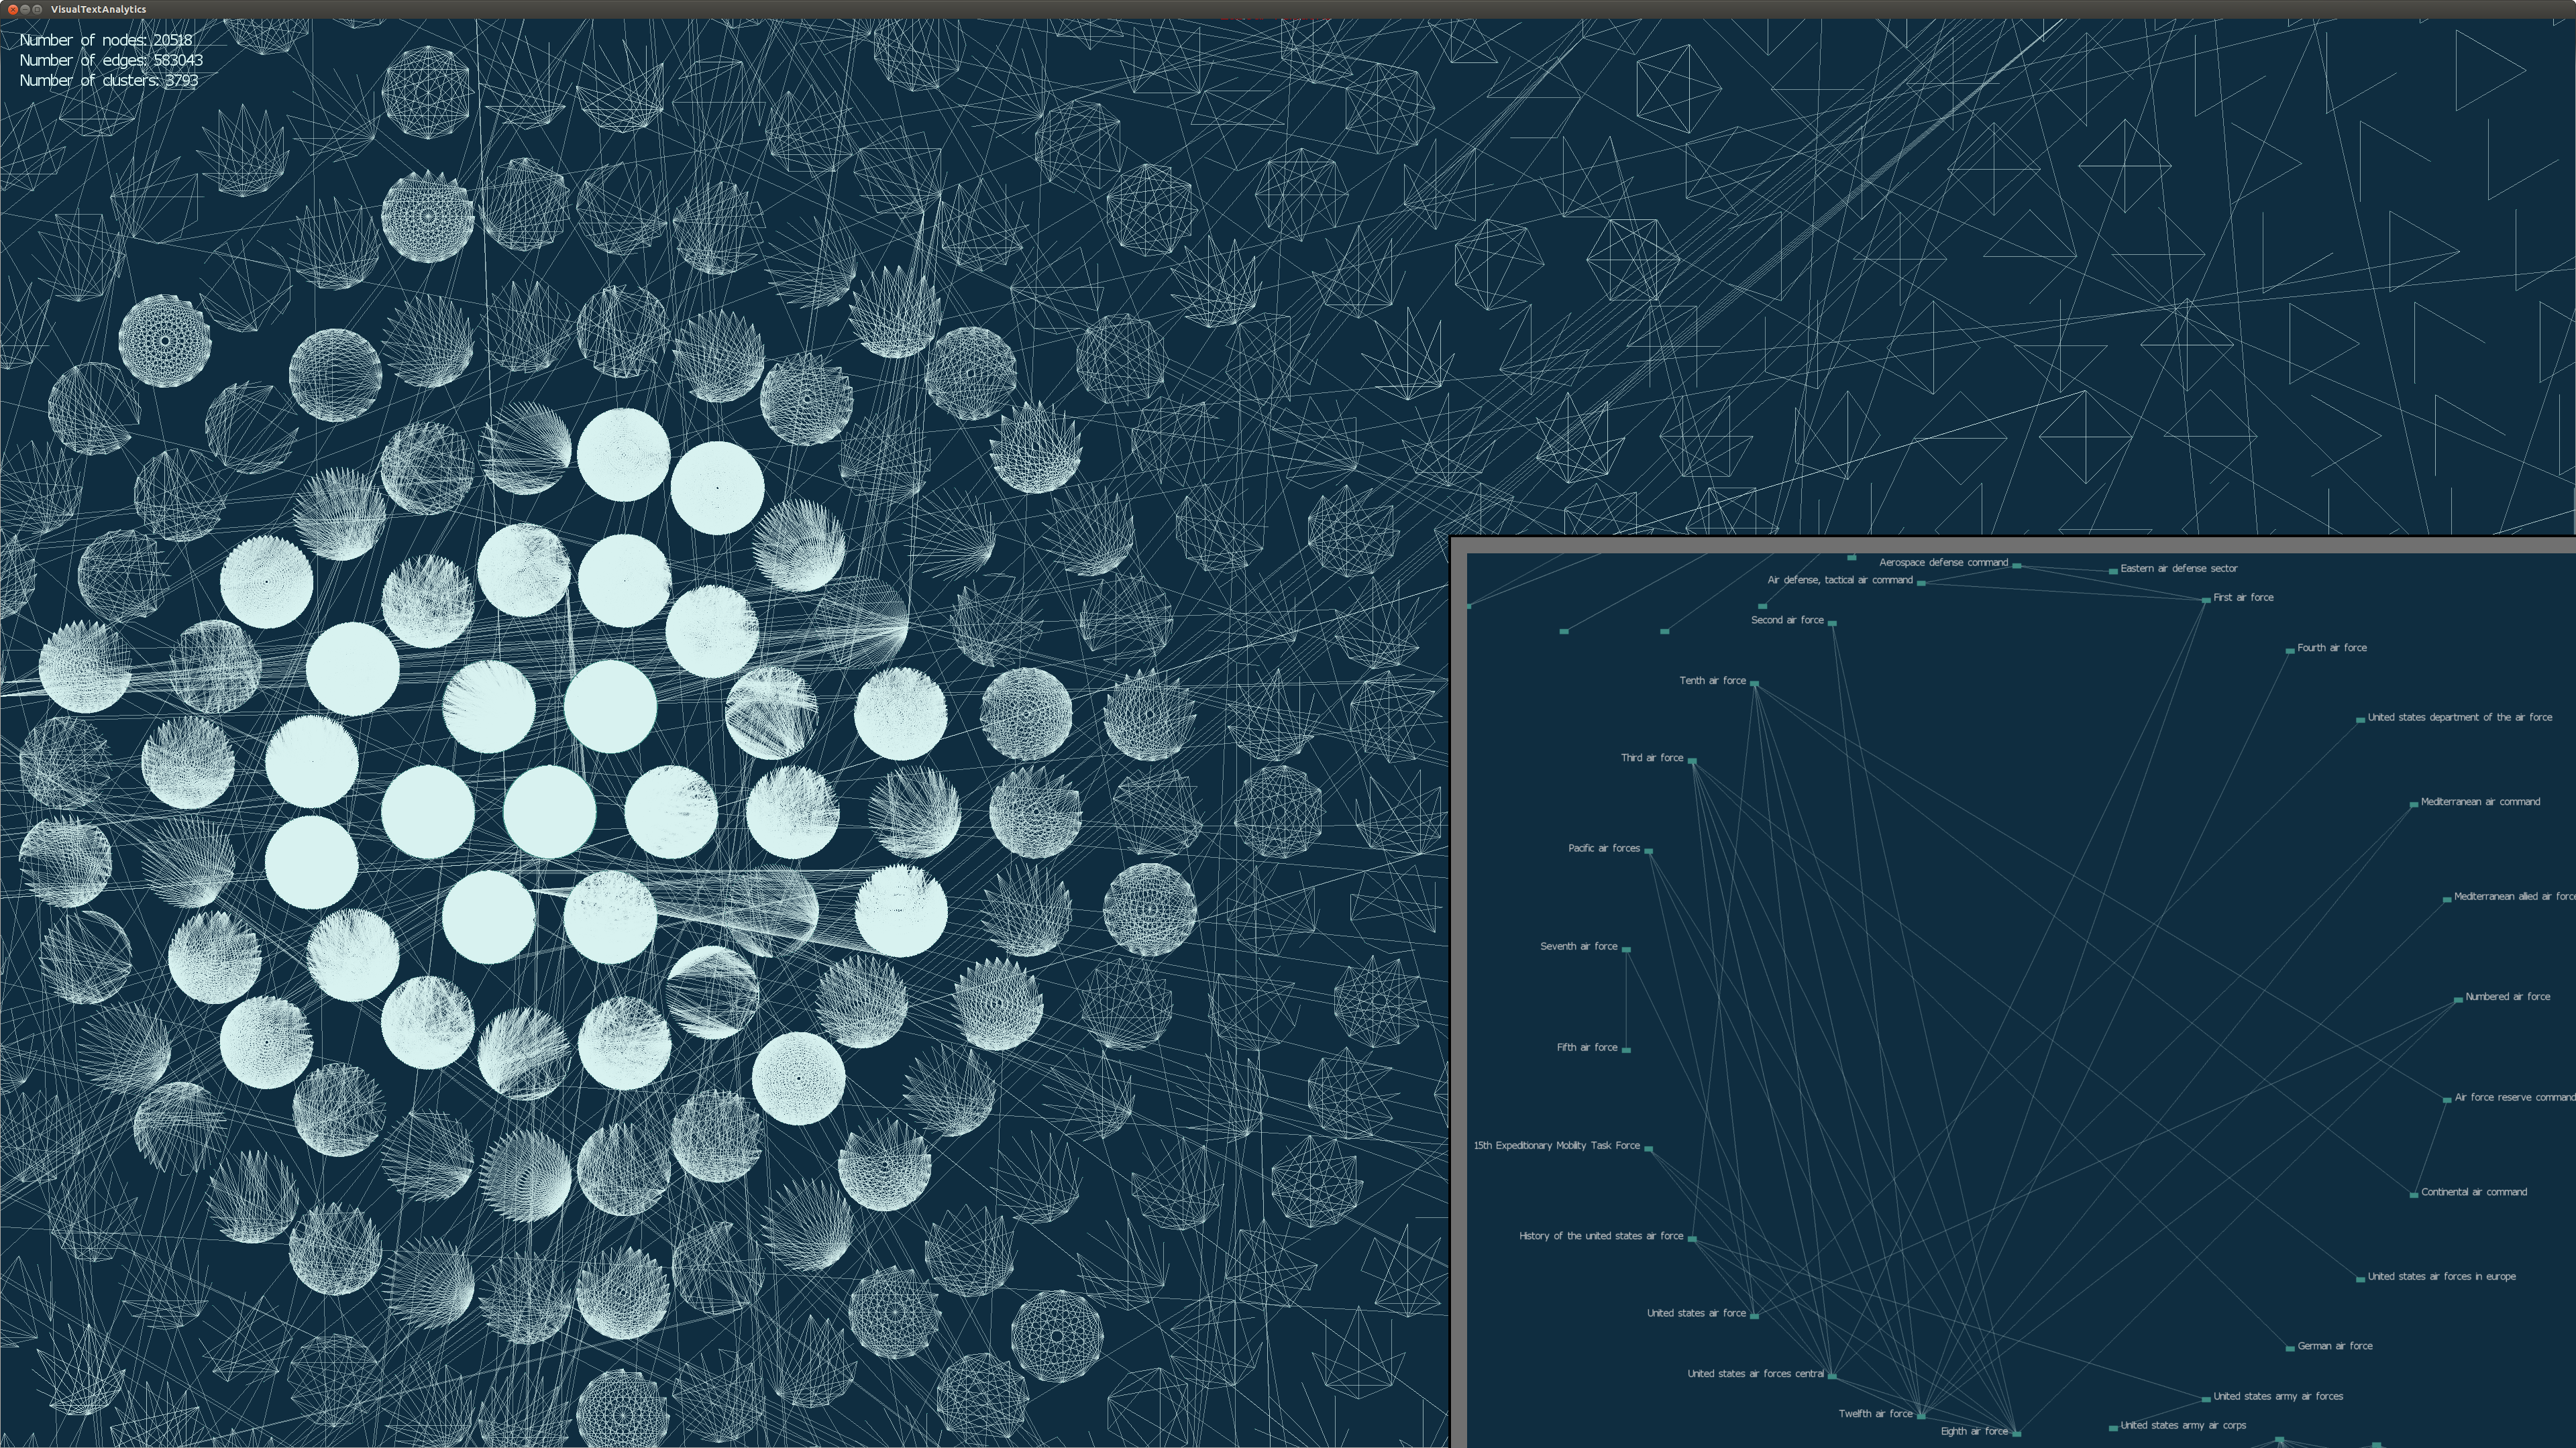
\includegraphics[width=\textwidth]{images/vta-cover}
\caption{Ausschnitt aus dem Projekt \textit{Visual Text Analytics}: In der unteren rechten Ecke ist ein Cluster im Fokus zu sehen. Der Hintergrund zeigt die Startvisualisierung mit einer Übersicht aller Cluster.}
\label{fig:vta-cover}
\end{figure}

Ergänzend wird eine zweite, die Darstellung der Artikel unterstützende, Visualisierung der zugehörigen Wikipedia-Kategorien als Graph bereitgestellt.
In dieser Darstellung werden Kategorien als Knoten abgebildet, die Kanten repräsentieren eine Verknüpfung von zwei Kategorien.
Der die Wikipedia-Kategorien abbildende Graph soll eine verständliche Zusammenfassung auf einer höheren Abstraktionsebene für die Menge der erfassten Wikipedia-Artikel ermöglichen, wie in der Abbildung \ref{fig:category-view} verdeutlicht.


\section{Problemstellung und Zielsetzung}
Die im Laufe des Projekts \emph{Visual Text Analytics} identifizierten Probleme geben den Anstoß für die Entwicklung einer neuen Herangehensweise an die Visualisierung.
Im Folgendem wird auf die für diese Arbeit relevanten Erkenntnisse kurz eingegangen.\\
Die Visualisierung der Artikelähnlichkeiten in Gruppen von Artikeln, sogenannten Artikelclustern, wird durch einen definierten Schwellwert erzeugt.
Der Schwellwert bestimmt, inwieweit die Ähnlichkeitsmatrix traversiert wird.
Die Herabsetzung des Schwellwerts durch den Nutzer führt zu einer steigenden Anzahl an zu traversierenden Artikelähnlichkeiten aus der Ähnlichkeitsmatrix.
Durch den herabgesetzten Schwellwert wird eine größere Anzahl von Artikelähnlichkeiten in Betracht gezogen.
Dies führt zu neu erzeugten Artikelclustern.
Für diese neu entstandenen Artikelcluster muss eine neue Visualisierung gezeichnet werden.
Da die Anzahl der zu betrachtenden Artikelähnlichkeiten gestiegen ist, steigt auch die Dauer der Berechnung der Anordnung der neuen Darstellung.
Die wachsende zeitliche Verzögerung führt dazu, dass die Visualisierung statisch wirkt, wodurch keine unmittelbare Interaktion zustande kommt.

\begin{figure}[H]
    \centering
    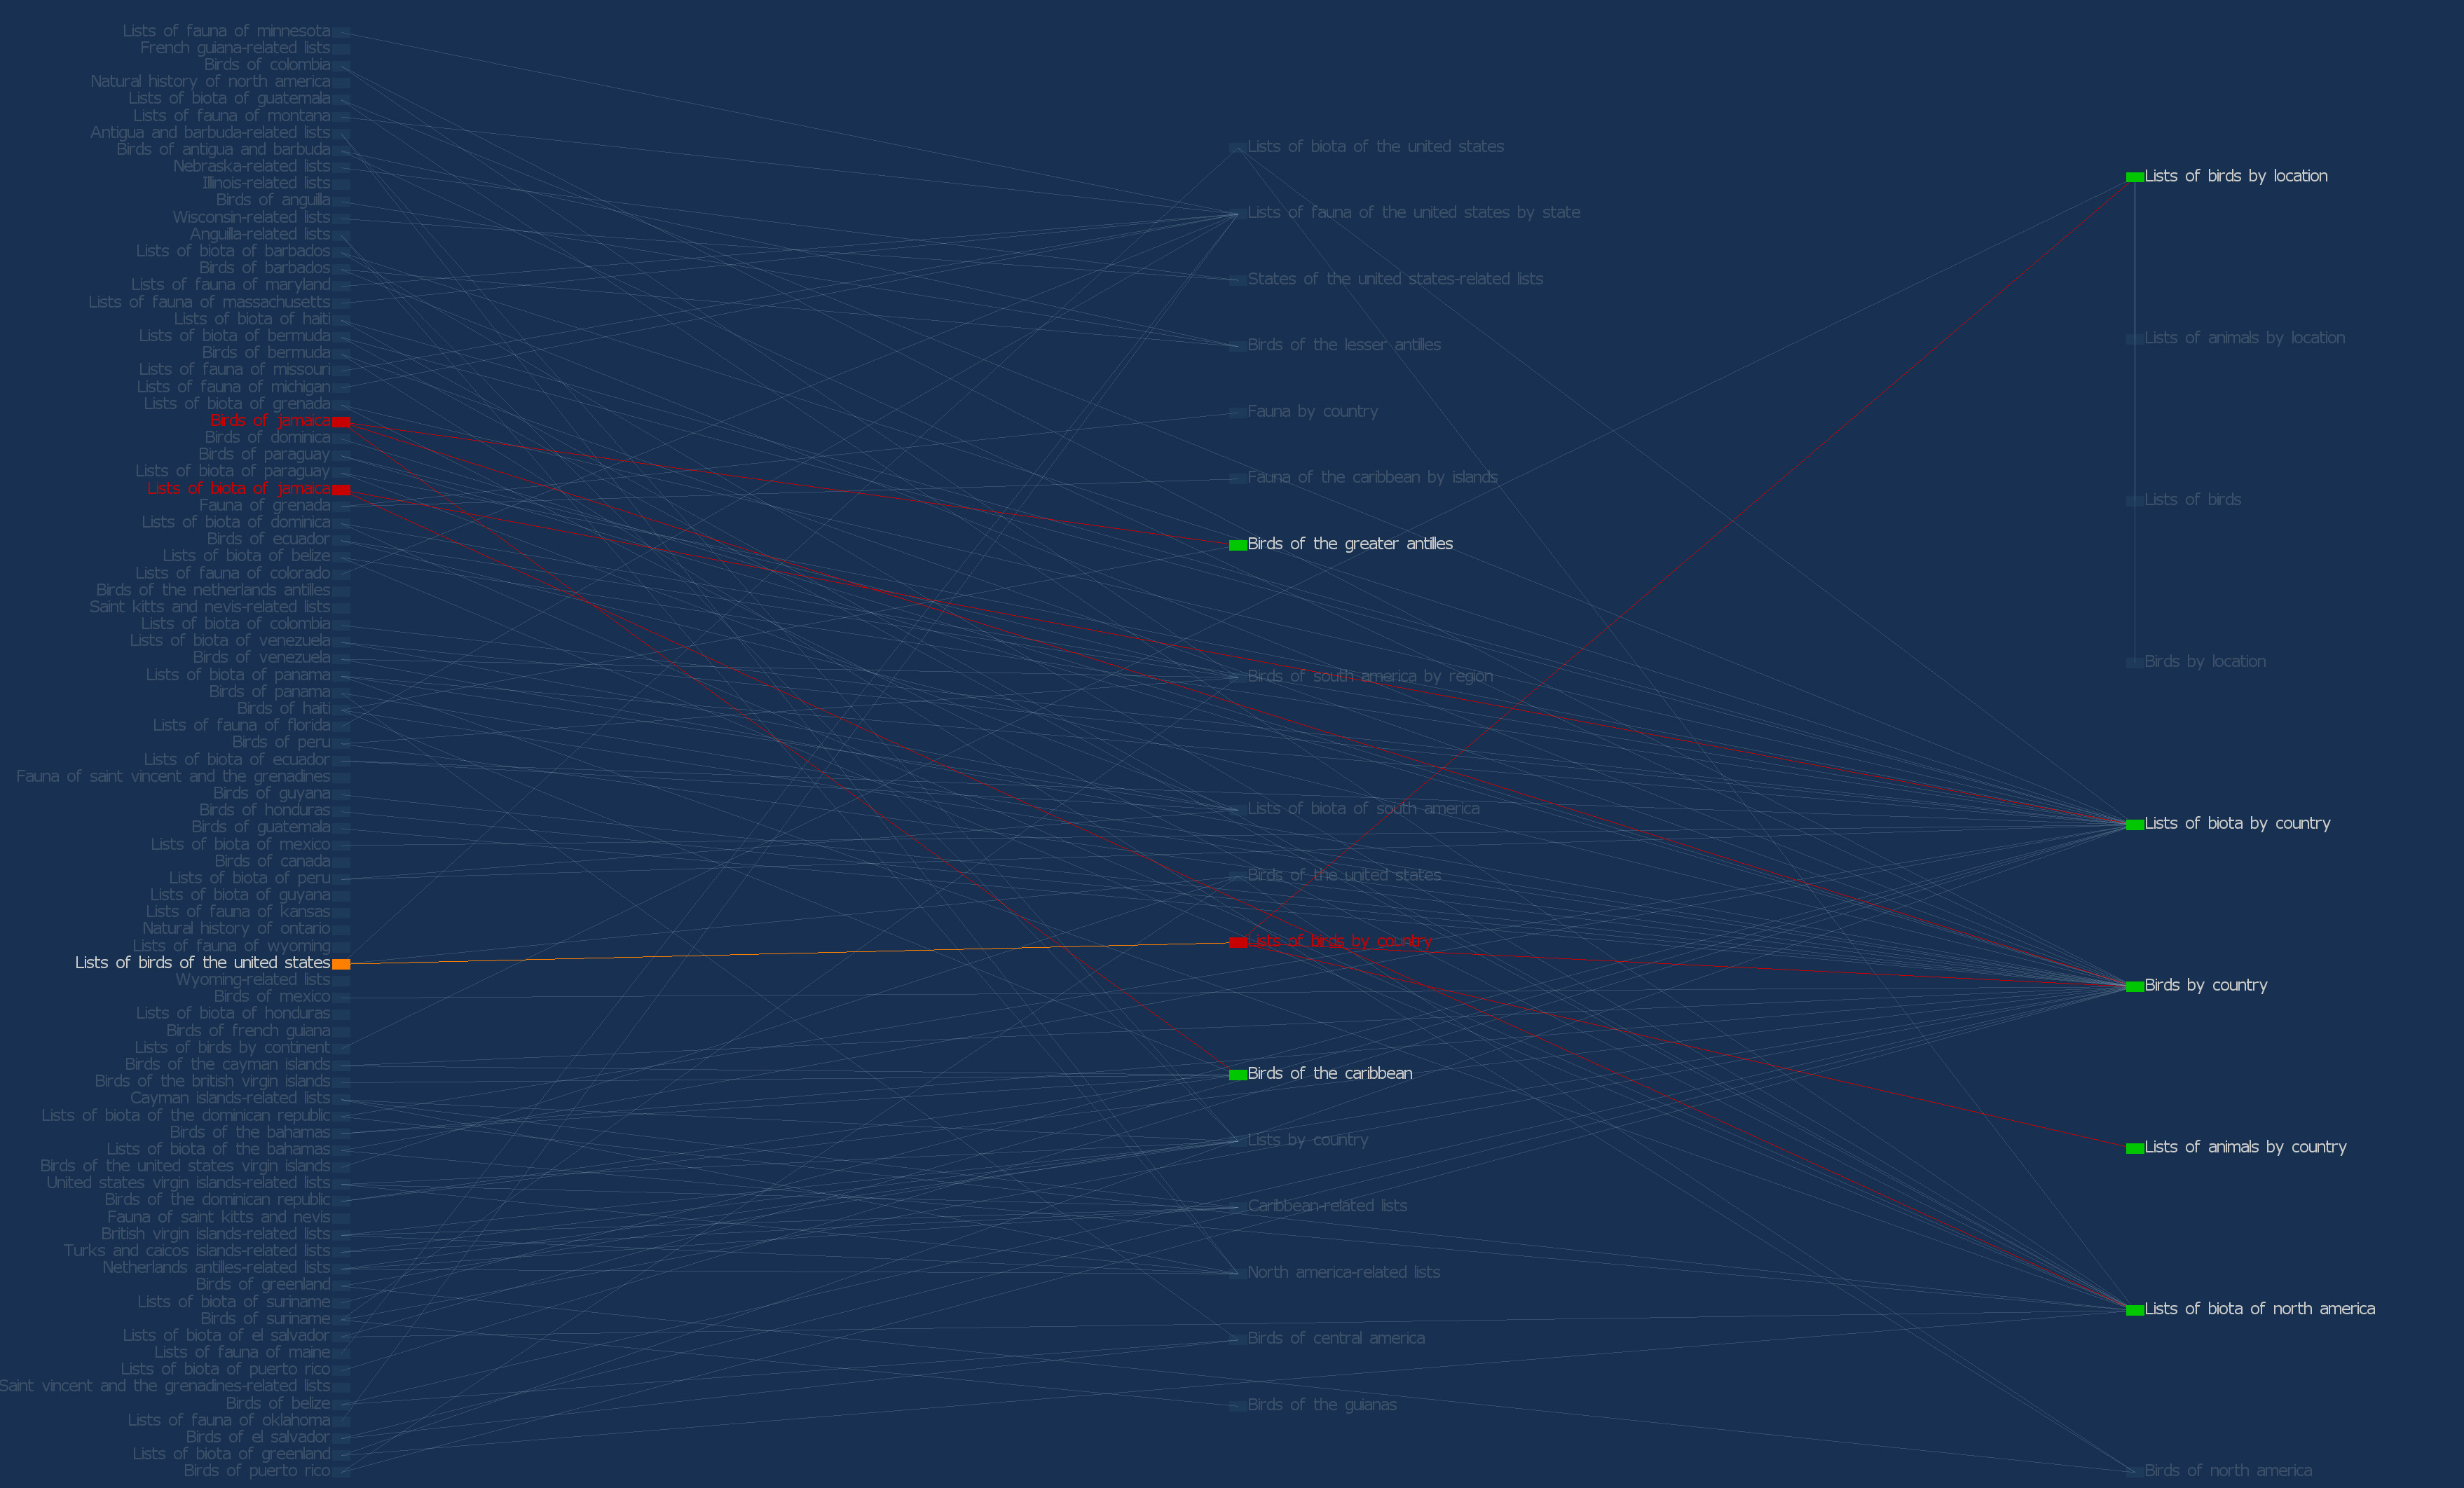
\includegraphics[width=\textwidth]{images/category-view}
    \caption{Ausschnitt des Kategoriengraphen: Die Knoten stellen Kategorien dar, die Kanten veranschaulichen die Verbindungen zwischen den Kategorien.\\ In diesem Bild wird die grün gefärbte Kategorie ausgewählt. Alle Knoten und Kanten ohne Verbindung zur ausgewählten Kategorie sind ausgegraut.}
    \label{fig:category-view}
\end{figure}

Um die zeitaufwendige Berechnung der Anordnung zu umgehen, können die Artikelähnlichkeiten, die durch den herabgesetzten Schwellwert einbezogen werden, der bestehenden Visualisierung in Form von Kanten hinzugefügt werden. 
Daraus resultiert jedoch eine massive Überzeichnung der Elemente, was folglich die Nachvollziehbarkeit der in der Visualisierung dargestellten Informationen erschwert.

Daraus lässt sich schließen, dass die Größe der Ähnlichkeitsmatrix Auswirkungen auf die Anordnung, das Verständnis und die Interaktivität der Visualisierung hat.
Aus den genannten Gründen sucht diese Arbeit nach einem Ansatz, die Größe der Ähnlichkeitsmatrix zu beeinflussen.\\
Der Fokus dieser Forschungsarbeit liegt im Gegensatz zur vorherigen Arbeit \emph{Visual Text Analytics} nicht auf den Artikeln, sondern auf den Kategorien der Wikipedia, mit deren Hilfe die Größe der Ähnlichkeitsmatrix reduziert und eine neue Form der visuellen Darstellung geschaffen wird.\\
Durch letztere soll ein neuer Zugang geschaffen werden, welcher die Verbindungen zwischen den Kategorien aufdeckt.
Zudem soll dem Nutzer der Visualisierung ermöglicht werden, nach allen verfügbaren Kategorien der Wikipedia zu suchen, die Verbindungen der Kategorien zueinander dynamisch zu erweitern und zu erforschen.
Diese interaktive Exploration der Visualisierung bildet den Mittelpunkt der vorliegenden Arbeit.



% ab hier nicht mehr relevant
%NOTE
% Relevanz von Informationsvisualisierung\\
% Bezug auf das vorangegangene Projekt Visual Text Analytics\\
% einmal eine Abstrakte Motivation -> Darstellung Kategorienbaum + "Ahnlichkeiten
%
% Motivation aus dem vorg"anger Projekt -> konkreter Bezug auf fehlende Eigenschaften und Erkenntnisse
% defacto die einzige Visualisierung f"ur den Kategoriebaum der Wikipedia
% =========================================================

% BULLET LIST ++++++++++++++++++++++++++++++++++++++++++++++++
% \begin{itemize}
%   \item Bedeutung des Wikipediadatensatzes
%   \item Kritikpunkte im Projekt Visual Text Analytics
%   \begin{itemize}
%     \item statisches Layout
%     \item fehlende M"oglichkeit zur Exploration der Daten
%     \item "Ubersicht der Visualisierung ist sehr undurchsichtig
%     \item Schwierigkeiten beim Nachvollziehen der Verbindungen zwischen den Artikeln untereinander
%     \item "Anderung des Schwellwertes f"ur "Ahnlichkeiten -> zu viele Kanten
%     \item fehlende M"oglichkeit, die Auswahl an Artikeln einzuschr"anken
%     \item Unterst"utzende Funktion zum Zusammenfassen von mehreren Artikeln -> Kategorien, Cluster
%     \item Artikelcluster mit vielen "Ahnlichkeiten zueinander sind schwer zu lesen
%     \item Kategorienbaum unzureichend als Unterzt"utzung neben den Artikeln
%   \end{itemize}
% \end{itemize}


% \begin{itemize}
%     \item Verbesserung des Verst"andnisses des "Ahnlichkeitsma"ses
%     \item Darstellung der Hierarchie von Kategorien
%     \begin{itemize}
%       \item Konstruktion eines Kategorienbaumes mit der M"oglichkeit der Exploration
%     \end{itemize}
%     \item Interaktive Visualisierung
%     \begin{itemize}
%       \item "Anderung des Schwellwerts zur Laufzeit
%     \end{itemize}
%     \item Exploration der Daten
%     \item Bezug zu anderen Datens"atzen: Autoren, Editierungen, etc.
% \end{itemize}
